\documentclass{article}
\usepackage[UTF8]{ctex}
% Replace `letterpaper' with`a4paper' for UK/EU standard size
\usepackage[a4paper,top=2cm,bottom=2cm,left=3cm,right=3cm,marginparwidth=1.75cm]{geometry}

% Useful packages
\usepackage{amsmath}
\usepackage{graphicx}
\usepackage[colorlinks=true, allcolors=blue]{hyperref}
\usepackage{graphicx} %插入图片的宏包
\usepackage{float} %设置图片浮动位置的宏包
\usepackage{subfigure} %插入多图时用子图显示的宏包
\usepackage{parskip}
\usepackage{indentfirst} 
\setlength{\parindent}{2em}
\usepackage{hyperref}  
\usepackage{tikz}
\allowdisplaybreaks
\usepackage{multirow}
\usepackage{amsmath}
\usepackage{amsfonts,amssymb} 
\usepackage{xcolor} % 用于显示颜色
\usepackage{listings} % 用于插入代码
\lstset{
	basicstyle          =   \sffamily,          % 基本代码风格
	keywordstyle        =   \bfseries,          % 关键字风格
	commentstyle        =   \rmfamily\itshape,  % 注释的风格,斜体
	stringstyle         =   \ttfamily,  % 字符串风格
	flexiblecolumns,                % 别问为什么,加上这个
	numbers             =   left,   % 行号的位置在左边
	showspaces          =   false,  % 是否显示空格,显示了有点乱,所以不现实了
	numberstyle         =   \zihao{-5}\ttfamily,    % 行号的样式,小五号,tt等宽字体
	showstringspaces    =   false,
	captionpos          =   t,      % 这段代码的名字所呈现的位置,t指的是top上面
	frame               =   lrtb,   % 显示边框
}

\lstdefinestyle{Python}{
	language        =   Python, % 语言选Python
	basicstyle      =   \zihao{-5}\ttfamily,
	numberstyle     =   \zihao{-5}\ttfamily,
	keywordstyle    =   \color{blue},
	keywordstyle    =   [2] \color{teal},
	stringstyle     =   \color{magenta},
	commentstyle    =   \color{red}\ttfamily,
	breaklines      =   true,   % 自动换行,建议不要写太长的行
	columns         =   fixed,  % 如果不加这一句,字间距就不固定,很丑,必须加
	basewidth       =   0.5em,
}

\title{数据结构第一次上机实验报告}
\author{林子开}
\begin{document}
	\maketitle
	\tableofcontents
\section{插入排序代码}
    \lstinputlisting[style = Python,
		caption={insertion sort 源代码},
		label = {insert}
		]{insertion_sort.py}

\section{merge排序代码}
    \lstinputlisting[style = Python,
		caption={merge sort 源代码},
		label = {merge}
		]{merge_sort.py}

\section{寻找最优的k}

\subsection{f(n,k)表达式的推导}
	在本节中,为方便讨论,如无特别说明,均考虑最差情况,即输入为降序排列的列表,输出为升序排列的列表。

	对于merge sort,设$T(n) = 2T(\frac{n}{2}) + dn$,则在递归的每一层中,merge过程的复杂度都为dn。

	对于insertion sort,由于我们已假设只考虑最差情况,则其时间复杂度为$g(n)=an^2+bn+c$,
	其中$a,b,c$均为常数。
	
	当列表长度小于或等于k时,就不再递归,直接调用插入排序。设递归开始时处在$\text{level}\,0$,
	并设假设在$\text{level}\,(m-1)$时$\frac{n}{2^{m-1}}>k$,在$\text{level}\,m$时
	$\frac{n}{2^{m}}\le k$,那么在$\text{level}\,m$时调用insertion sort。同时,可以知道$k$与$m$	
	满足的关系为:
	\begin{align} 
		k = \lceil \frac{n}{2^m} \rceil  \label{km1} \\
		m = \lceil \log_2(\frac{n}{k})  \rceil \label{km2}
	\end{align}
	
	画出对应的递归树如下:
	\begin{figure}[H]
		\centering  %图片全局居中
		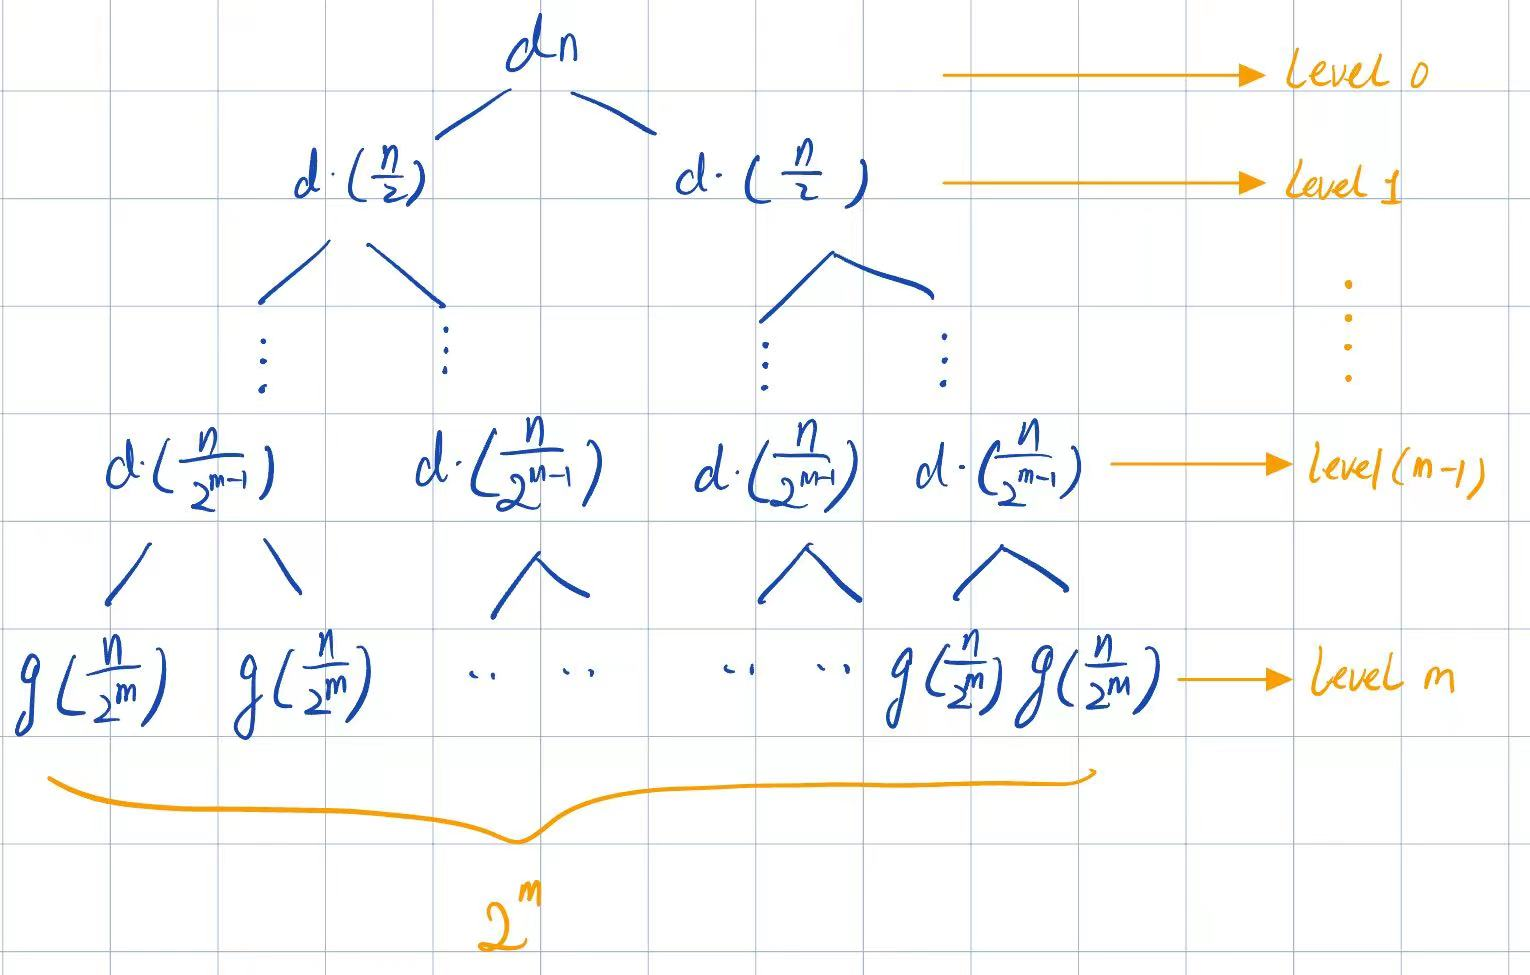
\includegraphics[width=0.8\textwidth]{递归树}
		\caption{combined sort 递归树}
	\end{figure}

	由递归树可以得到总的时间复杂度为
	\begin{align}
		f(n,m) &= dnm +  2^mg(\frac{n}{2^m})  \notag \\
		&= dnm + 2^m\left[a(\frac{n}{2^m})^2 + b(\frac{n}{2^m}) +c\right]
	\end{align}
	将式\eqref{km1} \eqref{km2}代入,在考虑渐进情况下的复杂度时,可忽略取整,于是得到:
	\begin{align}
		f(n,k) &= dn(\log_2n - \log_2k) + (\frac{n}{k})(ak^2 + bk +c)  \notag \\
			   &= dn\log_2n - dn\log_2k + ank + nb + \frac{nc}{k} 
	\end{align} 

\subsection{理论推导最优k}
	下面从理论上寻找最优的$k$。当$n$既定时,将$f(n,k)$对$k$求偏导得到:
	\begin{align}
		\frac{\partial f}{\partial k} 
		&= -dn\frac{1}{k}\log_2\text{e} + an - \frac{nc}{k^2} \notag  \\
		&= \frac{1}{k^2}(ank^2 - dn\log_2\text{e}k - nc) \label{k-partial}
	\end{align}
	其中e是自然对数的底。
	
	由式\eqref{k-partial},结合二次函数性质可知,在$k\ge 0$时只有一个极值点,而且是极小值点,该极值点为:
	\begin{equation}
		k^* = \frac{dn\log_2\text{e} + \sqrt{(dn\log_2\text{e})^2 - 4acn^2}}{2an} \label{bestK} \\
	\end{equation}
	
	则理论上当$k=k^*$时,在渐进情况下,算法会有最快的速度。

\subsection{实验寻找最优k}
	在实际情况下,由于常数$a,b,c,d$并不知道,所以需要通过实验来确定最优的$k^*$。
	在实验中,还需要测试平均情况(多组随机输入求平均值),以及最坏情况(倒序输入)。
	我们把可行的实验途径罗列如下,共四种:
	\begin{enumerate}
		\item \textbf{求常数+最坏情况}。对insert sort和merge sort取不同的n,分别输入长度为n的倒序数组并记录时间,
			再通过线性回归的方式估计最坏常数$a,b,c,d$,带回表达式\eqref{bestK},得到最优k。
		\item \textbf{求常数+随机情况}。对insert sort和merge sort取不同的n,分别多次输入长度为n的随机数组并求时间的平均值,
			再通过线性回归的方式估计随机情况下的常数$a,b,c,d$,带回表达式\eqref{bestK},得到最优k。
			但此方法不够稳定,可能会受伪随机数生成规律的影响而不准确。
		\item \textbf{固定n+最坏情况}。固定数组大小n,输入长度为n的倒序数组,尝试不同的k值并记录时间,找到时间最短的k。
		\item \textbf{固定n+随机情况}。固定数组大小n,多次输入长度为n的随机数组,尝试不同的k值并记录平均时间,找到平均时间最短的k。
			同样,此方法不够稳定,可能受伪随机数生成规律的影响。
	\end{enumerate}
	
	在本次报告中,我们只进行第3和第4类实验。
	
	我们考虑$n=100,250,500,1000$四种情况,输入最坏情况的倒序数组寻找使运行时间最短的k,
	以及输入多个随机排序数组并求平均时间最短的k,共八个实验,结果如下:

	\begin{figure}[H]
		\centering  %图片全局居中
		\subfigure[n=100, best k=1]{
			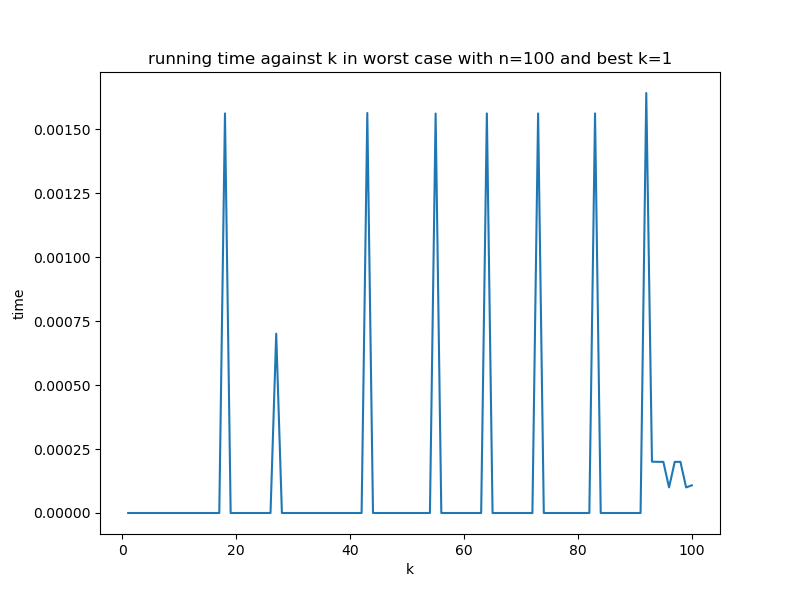
\includegraphics[width=0.45\textwidth]{worst case with n=100.png}}
		\,
		\subfigure[n=250, best k=2]{
			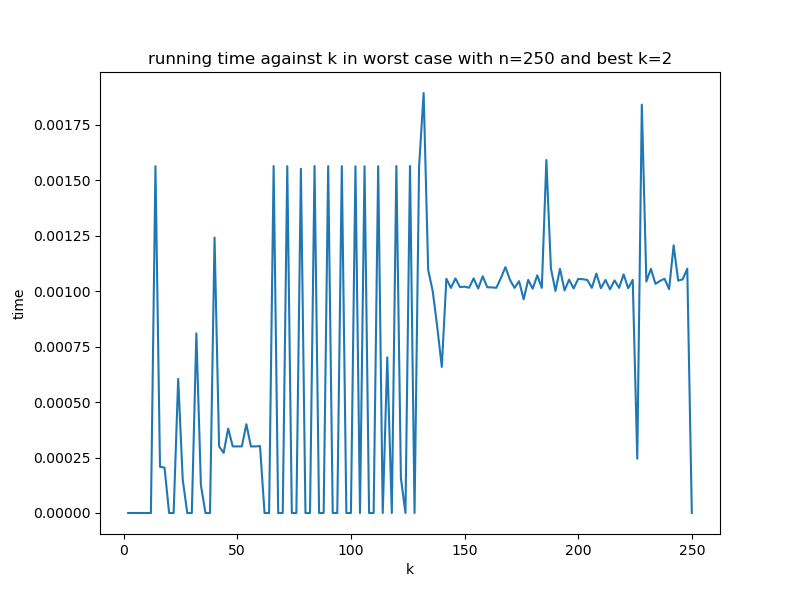
\includegraphics[width=0.45\textwidth]{worst case with n=250.png}}
		\,
		\subfigure[n=500, best k=2]{
			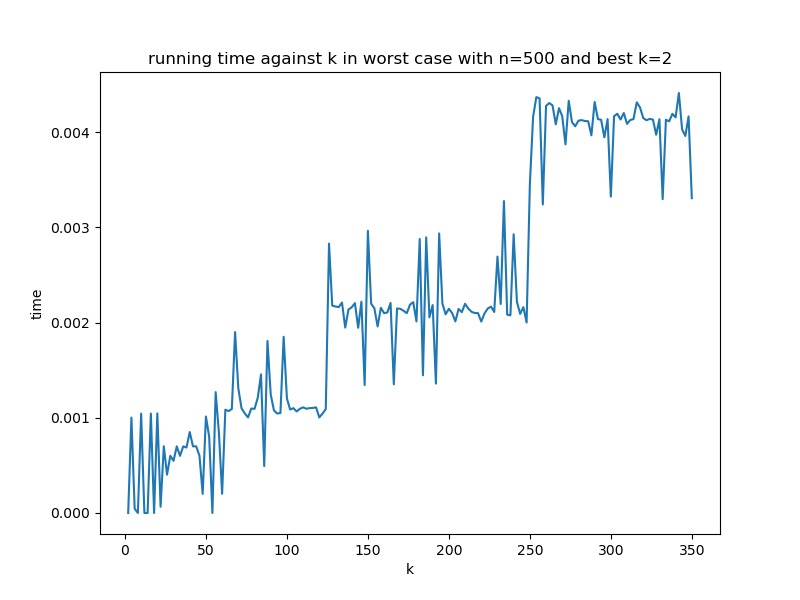
\includegraphics[width=0.45\textwidth]{worst case with n=500.png}}
		\,
		\subfigure[n=1000, best k=10]{
			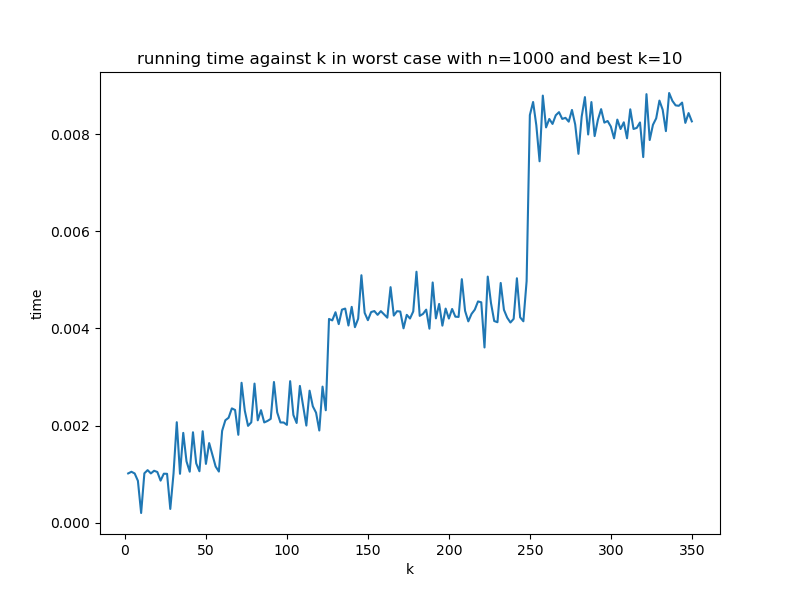
\includegraphics[width=0.45\textwidth]{worst case with n=1000.png}}
		\,
		\caption{在最坏倒序数组的情况下寻找最优k}
	\end{figure}

	\begin{figure}[H]
		\centering  %图片全局居中
		\subfigure[n=100, best k=1]{
			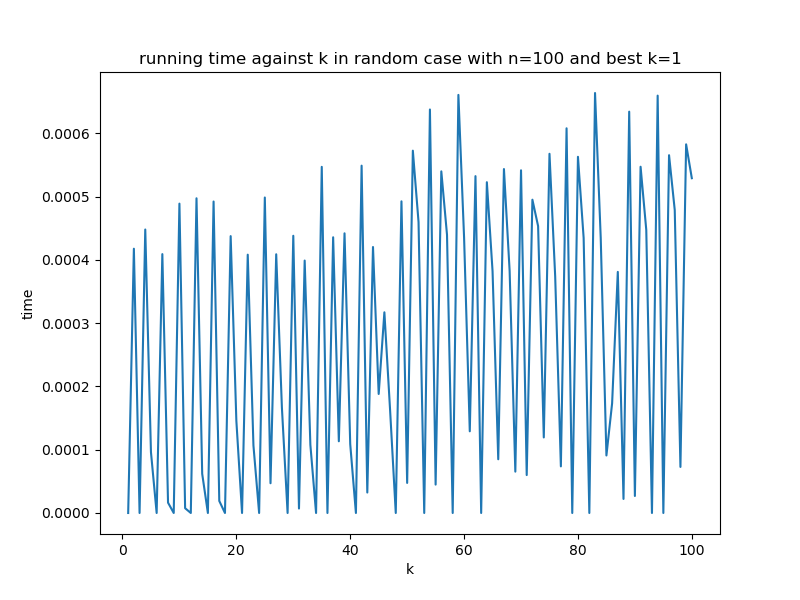
\includegraphics[width=0.45\textwidth]{random case n=100.png}}
		\,
		\subfigure[n=250, best k=10]{
			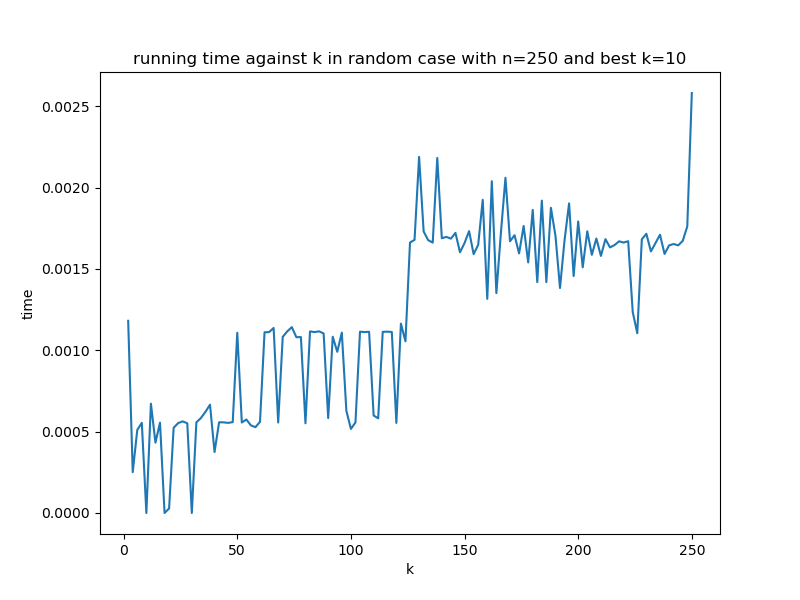
\includegraphics[width=0.45\textwidth]{random case n=250.png}}
		\,
		\subfigure[n=500, best k=16]{
			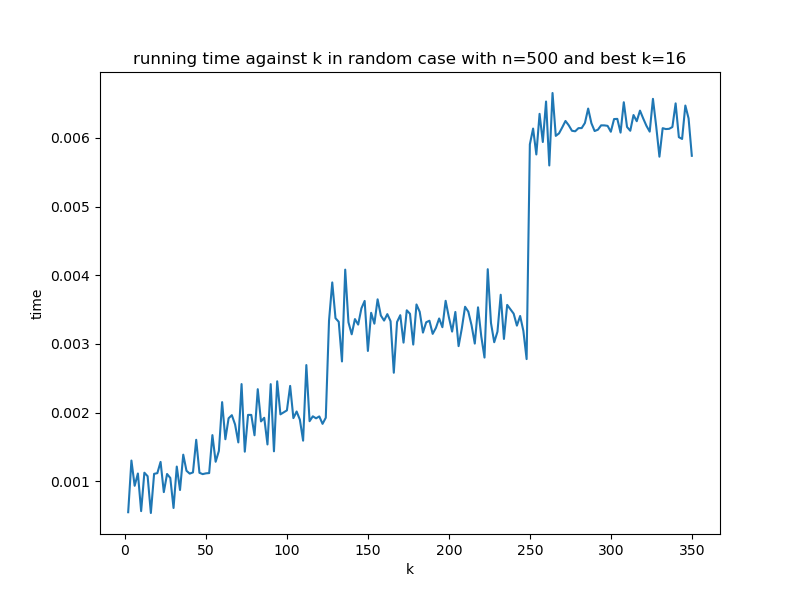
\includegraphics[width=0.45\textwidth]{random case n=500.png}}
		\,
		\subfigure[n=1000, best k=10]{
			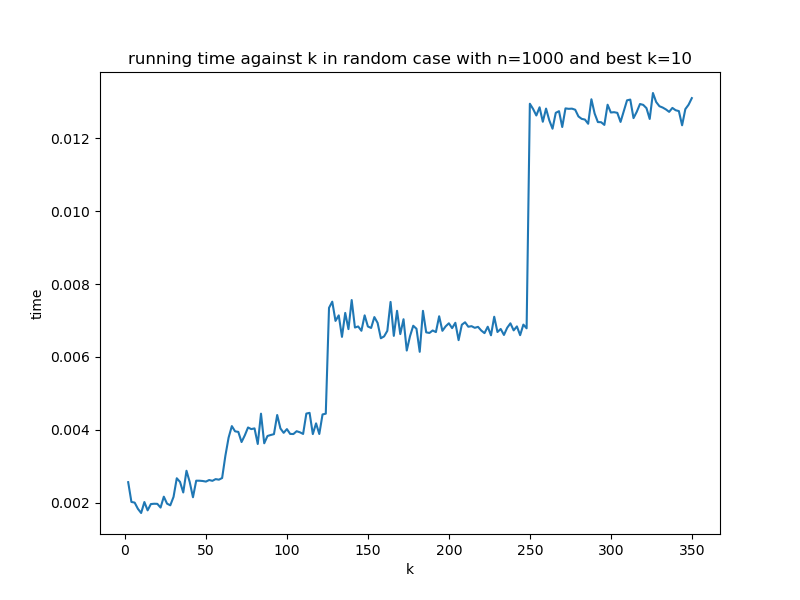
\includegraphics[width=0.45\textwidth]{random case n=1000.png}}
		\,
		\caption{在多个随机排序数组的情况下寻找使平均时间最短的k}
	\end{figure}

	可以发现,在随机情况下,k并没有明显随着n的增大而增大。
	

\section{融合后的排序代码}
	\lstinputlisting[style = Python,
	caption={combined sort 源代码},
	label = {combined},
	linerange={6-48}]{combined_sort.py}



\end{document}